\chapter{Statistiken}

    \section{Zahlen}
        \begin{itemize}
            \item Lines of Code: ca. 15000
            \item Commits: ca. 370
        \end{itemize}
        
    \section{Graphen und Statistiken}
    Abschließend sind folgend ein paar Graphen aus GitHub und gitstats abgebildet, die die Verteilung von Commits und Zeilen Code pro Autor darstellen. Die Graphen werden durch die hohe Anzahl an Zeilen Einzelner, die viel automatisch generiert haben, leicht verfälscht. Insgesamt kann man erkennen, dass die Arbeitsaufteilung ungefähr gleich ist.

		\begin{figure}[ht] 
			\centering
			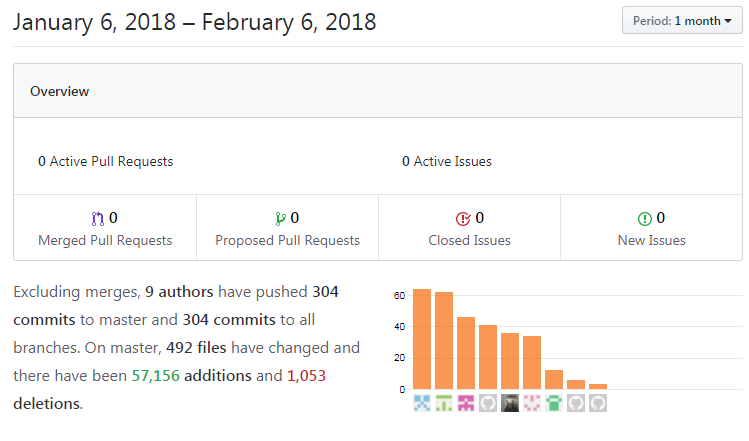
\includegraphics[scale=0.70, trim= 1cm 0 0 0]{pulse.png}
            \caption{GitHub Insights - Pulse}
			\label{fig1}
		\end{figure}

		\begin{figure}[ht] 
			\centering
			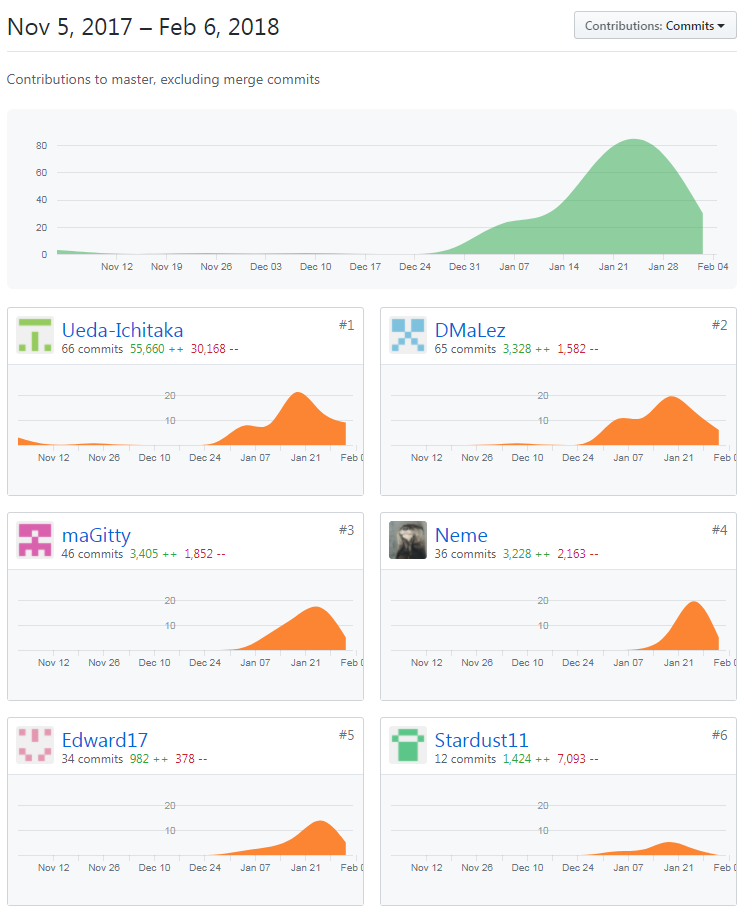
\includegraphics[scale=0.70, trim= 1cm 0 0 0]{contributors.png}
            \caption{GitHub Insights - Contributors}
			\label{fig2}
		\end{figure}

		\begin{figure}[ht] 
    		\centering
			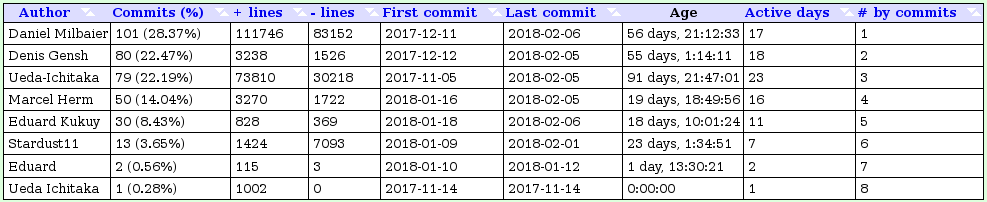
\includegraphics[scale=0.7, trim= 3cm 0 0 0]{authors.png}
            \caption{GitStats - List of Authors}
			\label{fig3}
		\end{figure}
	
		\begin{figure}[ht] 
			\centering
			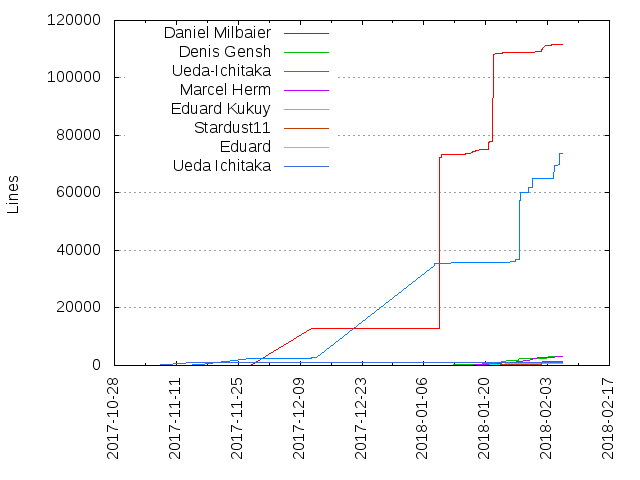
\includegraphics[scale=0.80, trim= 1cm 0 0 0]{lines_of_code_by_author.png}
            \caption{GitStats - Lines of Code per Author}
			\label{fig4}
		\end{figure}

		\begin{figure}[ht] 
			\centering
			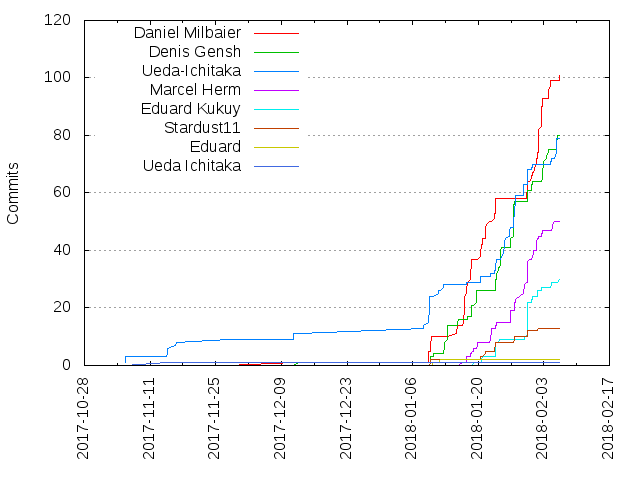
\includegraphics[scale=0.80, trim= 1cm 0 0 0]{commits_by_author.png}
            \caption{GitStats - Commits per Author}	
			\label{fig5}
		\end{figure}
